\section{\label{sec:sim}Simulations}

All the programs in this section can be obtained from the standard \desg{SVN} repository for \desg{CLAS} here:
\begin{center}
    \url{https://jlabsvn.jlab.org/svnroot/clas/trunk}
\end{center}
Under this directory, you may find the following directories which hold the programs in the order which they appear below:
\begin{itemize}
    \item \prog{simulation/generators/genr8}
    \item \prog{io/part2gamp}
    \item \prog{io/bosdump}
    \item \prog{simulation/generators/ppgen}
    \item \prog{simulation/gsim}
    \item \prog{simulation/gpp}
\end{itemize}

\subsection{\label{sec:sim.gen}Generating Events for Digitization}

One may use the program \texttt{genr8} for generating t-channel phase space events. It is driven by an input key file which describes the exclusive reaction. Typical usage to generate 10k events from 4.4 to 5.45~GeV in beam energy using the input file ``\verb+n_pi-pi+pi+.input+'' looks like this:
\begin{verbatim}
genr8 -M10000 -B4.4,5.45 -oevents.gamp < n_pi-pi+pi+.input
\end{verbatim}
See the genr8 documentation for how to write the input file, or you can see this example here:
\begin{align}
    \texttt{http://clasweb.jlab.org/rungroups/g12/wiki/index.php/N\_pimpippip} \nonumber
\end{align}

Gsim requires a bos file with a PART bank containing the MC event. Note PART bank 0 is reserved for MC events whereas PART banks 1 and 2 are used for containing the reconstructed event. The best way to convert GAMP to PART banks is by using gamp2part -- the command, for protons pions and kaons, following the example above is:
\begin{verbatim}
gamp2part -r56855 -oevents.part -T -S-0.321,0.378,-0.254,0.407 \
  -z-110,-70 events.gamp
\end{verbatim}
and for electrons and positrons
\begin{verbatim}
gamp2part -r10 -oevents.part -T -S-0.321,0.378,-0.254,0.407 \
  -z-110,-70 events.gamp
\end{verbatim}
where the option -r10 is specific to RUN 10 in:
\begin{verbatim}
export CLAS_CALDB_RUNINDEX=calib_user.RunIndexg12_mk
\end{verbatim}
This writes a BOS file full of PART, sector 0 banks with the 4-vector information from the gamp file. Also, the -z option smears the target distribution in Z, while the -S smears it in X and Y. The parameters are means and sigmas of a 2D Gaussian which were derived from a fit to the data. An alternative way to convert a gamp file to a BOS PART bank file is using gamp2txt and txt2part. These programs are piped together during run time.
\begin{verbatim}
gamp2txt -E5.714 -z-110,-70 < events.gamp | txt2part -T -oevents.part
\end{verbatim}
The above command takes in gamp events, smears the z vertex in the target range, creates a tagger hit and writes out a bos file with HEAD, PART, and TAGR banks. Here is a bosdump of an event:
\begin{verbatim}
ifarml1> bosdump events.part -M1
Group:  HEAD    Sector: 0       Nhits:  1   Next ind:    0

Version:        0
Run:            1
Event:          1
Type:           -2  (GSIM monte carlo)
ROC:            0
CLASS:          15
Trgbit:         0x1
TIME:           Wed Feb 27 22:16:00 2008


Group:  PART    Sector: 0       Nhits:  3  Next ind:       0
pid:   8
   vert-> x: 0.000  y: 0.000  z: -95.178
   p-> E: 3.194  px: -0.591  py: -0.688  pz: 2.942
   q: 1.000  trkid:   0  qpid: 0.000  qtrk:  0  flags:   0
pid:   9
   vert-> x: 0.000  y: 0.000  z: -95.178
   p-> E: 3.194  px: -0.591  py: -0.688  pz: 2.942
   q: -1.000  trkid:   0  qpid: 0.000  qtrk  0  flags:   0
pid:   8
   vert-> x: 0.000  y: 0.000  z: -95.178
   p-> E: 4.780  px: -0.246  py: -0.140  pz: 4.383
   q: 1.000  trkid:   0  qpid: 0.000  qtrk:   0  flags:   0

Group:  TAGR    Sector: 0       Nhits:  1  Next ind:      0
ERG:5.001 TTAG:0.000  TPHO:0.000 STAT:15 T_id:17  E_id:82
\end{verbatim}

One can use any alternative to \texttt{genr8} as long as the output is either gamp or an appropriate BOS file. For example, there is the phase-space generator \texttt{ppgen}:
\begin{verbatim}
ppgen -M<reaction code> -P<photon energy> -E5.714 -j1 -G -A \
  -t<t-slope> -m50000 > events.gamp
\end{verbatim}
The output can be txt or gamp file depending on user's needs. Follow the previous instructions to convert to part banks as needed.

\subsection{\label{sec:sim.digit}Digitization and Smearing}

The program to track the particles through the simulation and ultimately digitize the information to simulated ``raw'' banks is the geant3-based program: \texttt{gsim}. Running this on the BOS file created above looks like this:
\begin{verbatim}
gsim_bat -ffread ffread.g12 -kine 1 -mcin events.part \
  -bosout events.gsim -trig 2000000
\end{verbatim}
Using the above command, should create a gsim BOS output file. Here is the FFREAD file should be used to run gsim\_bat for \desg{g12} analyses not using electrons/positrons:
\begin{verbatim}
===BEGIN=====FFREAD.G12======================
CUTS   5.e-3 5.e-3 5.e-3 5.e-3 5.e-3
DCCUTS 1.e-4 1.e-4 1.e-4 1.e-4 1.e-4
ECCUTS 1.e-4 1.e-4 1.e-4 1.e-4 1.e-4
SCCUTS 1.e-4 1.e-4 1.e-4 1.e-4 1.e-4

MAGTYPE 2
MAGSCALE 0.500 0.000
PTGIFIELD 0
STTYPE 1
STZOFF -90.0
TGPOS 0. 0. 0.
TARGET 'g11a'
TGMATE 'PROT'
POSBEAM 0.0 0.0

GEOM 'ALL' 'ST'
NOGEOM 'MINI' 'PTG '
BEAM 0 0 5.714
DCAY 1
KINE 1
MULS 1
AUTO 1

RUNG 56855
TIME 1000000 1000000 1000000
TRIG 1000000
STOP
===END=====FFREAD.G12=======================
\end{verbatim}
and for electrons/positrons the FFREAD file should read
\begin{verbatim}
=============FFREAD.G12======================
CUTS   5.e-3 5.e-3 5.e-3 5.e-3 5.e-3
CCCUTS 1.e-3 1.e-3 1.e-3 1.e-3 1.e-3
DCCUTS 1.e-4 1.e-4 1.e-4 1.e-4 1.e-4
ECCUTS 1.e-4 1.e-4 1.e-4 1.e-4 1.e-4
SCCUTS 1.e-4 1.e-4 1.e-4 1.e-4 1.e-4

UPSTPOS 0. 0. 0.
MAGTYPE 2
MAGSCALE 0.500 0.000
PTGIFIELD 0
STTYPE 1
STZOFF -90.0
TGPOS 0. 0. 0.
TARGET 'g11a'
TGMATE 'PROT'
POSBEAM 0.0 0.0
GEOM 'ALL' 'ST'
NOGEOM 'MINI' 'PTG'
BEAM00 5.714
DCAY 1
PAIR 1
HADR 1
MULS 1
KINE 1
AUTO 1
RUNG 10
TRIG 200000
STOP
============================================
\end{verbatim}
The tracking and digitization done by \texttt{gsim} is ideal and there is no smearing done. To get the simulated data to mimic the detector resolution the ``gsim post-processor'' (\texttt{gpp}) is used. For \desg{g12}, and following the above example, one should use this command for protons, pions and kaons:
\begin{verbatim}
gpp -Y -s -S -a2.73 -b1.7 -c1.93.-f1 -R56855 -P0x7f -oevents.gpp events.gsim
\end{verbatim}
and for electrons and positrons
\begin{verbatim}
gpp -Y -s -S -a2.73 -b1.7 -c1.93.-f1 -R10 -P0x7f -oevents.gpp events.gsim
\end{verbatim}
The values passed to the gpp command line options, -a, -b, -c, helps match the tracking resolution of the simulated data to that of the real events in the regions 1,2 and 3 of the CLAS Drift Chambers. They accomplish this by smearing the DOCA values and hence gpp is able to match the DC residuals for the simulated CLAS tracks to that of the real CLAS tracks on a region-by-region basis. The gpp option -f smears the Time-of-Flight tdc values and during analysis the default gpp smearing for TOF was found to be adequate. The smearing should be run with a good g12 run number; run 56855 has all the necessary constants in the database to get the tagger timing smearing done correctly. Also, interested parties can add accidentals to the TAGR bank by using the -A option like so:
\label{cmd:gppAoption}\begin{verbatim}
gpp -Y -s -S -a2.73 -b1.7 -c1.93 -f1 -R56855 -P0x7f -oevents.gpp \
  -A/path/to/output/from/filter_tagr events.gsim
\end{verbatim}
The program \texttt{filter\_tagr} scans through real data files and outputs a bos file containing only the TAGR banks. These files are then supplied to gpp with the -A option, and gpp puts the contents of these banks as accidentals in the MC TAGR bank. Output from \texttt{filter\_tagr} for run 56855 can be found at:
\begin{align}
    \texttt{/home/clasg12/local/etc/clas6/gpp\_tagger\_profile.bos} \nonumber
\end{align}


As stated earlier, the goal of using GPP is to simulate the experimental conditions as close as possible. So we smear the values of the DOCA for the simulated tracks with a single Gaussian whose width is equal to the events weighted sum of the widths of the two Gaussians fitted to the data from the run 56855. This makes the residual for a superlayer in the simulated data approximately equal to the weighted residual from the real data. The default available options for GPP specifies only three parameters `-a, -b, -c' for DC DOCA smearing, where each parameter is responsible for the smearing of two superlayers (in one Region) of all six sectors. Hence, we choose a set of parameters based on the following fits as seen in Figs.~\ref{fig:SLRes} and \ref{fig:SLRes_default}, which gives us the best match on average between the different superlayers in the six sectors (see Fig.~\ref{fig:DC_SL_Match}).

\begin{figure}[htpb]\begin{center}
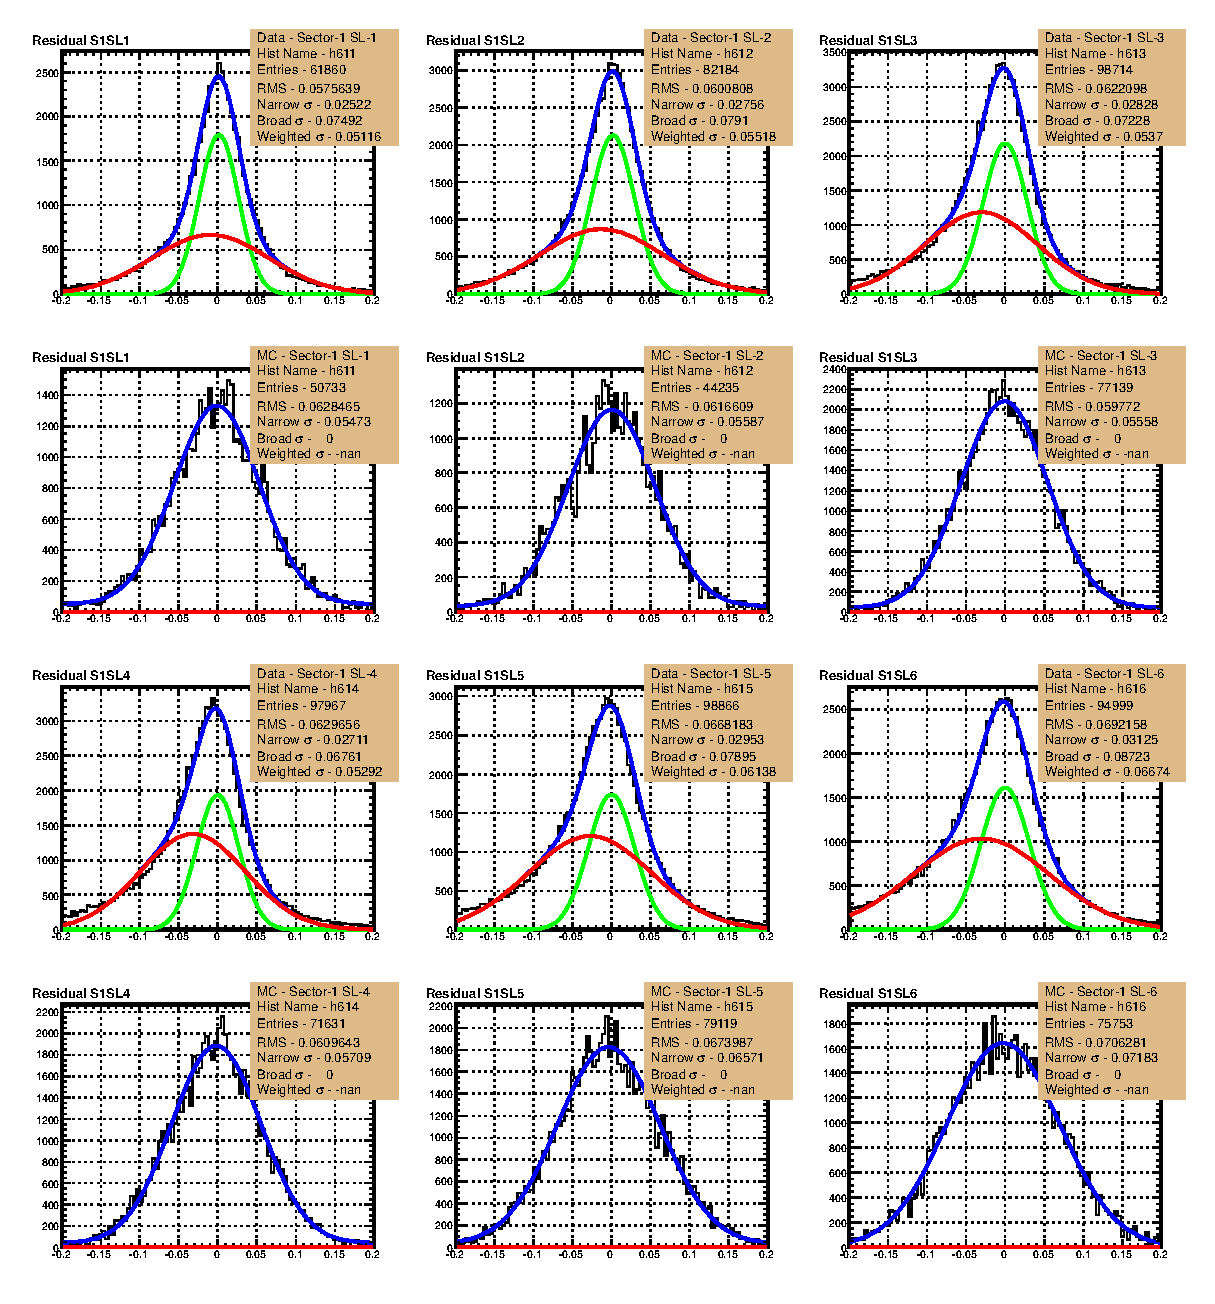
\includegraphics[width=0.8\columnwidth]{figures/calib/dc/Sector_1_compare.eps}
\caption[DC superlayers Resolution Matching]{\label{fig:SLRes}Plots and Fits used to match the residuals (resolution) for Drift Chamber superlayers in CLAS Sector 1, between the Data and the Simulation. Data is an empirical fit to a convolution of two gaussians. The simulated distribution is a single gaussian with its simulated width approximately equal to the weighed sum of the widths of the two gaussians fitted to the data. This simulation uses the best estimated smearing parameters to match the DC residuals, between the Data and the Simulation.}
\end{center}\end{figure}

\begin{figure}[htpb]\begin{center}
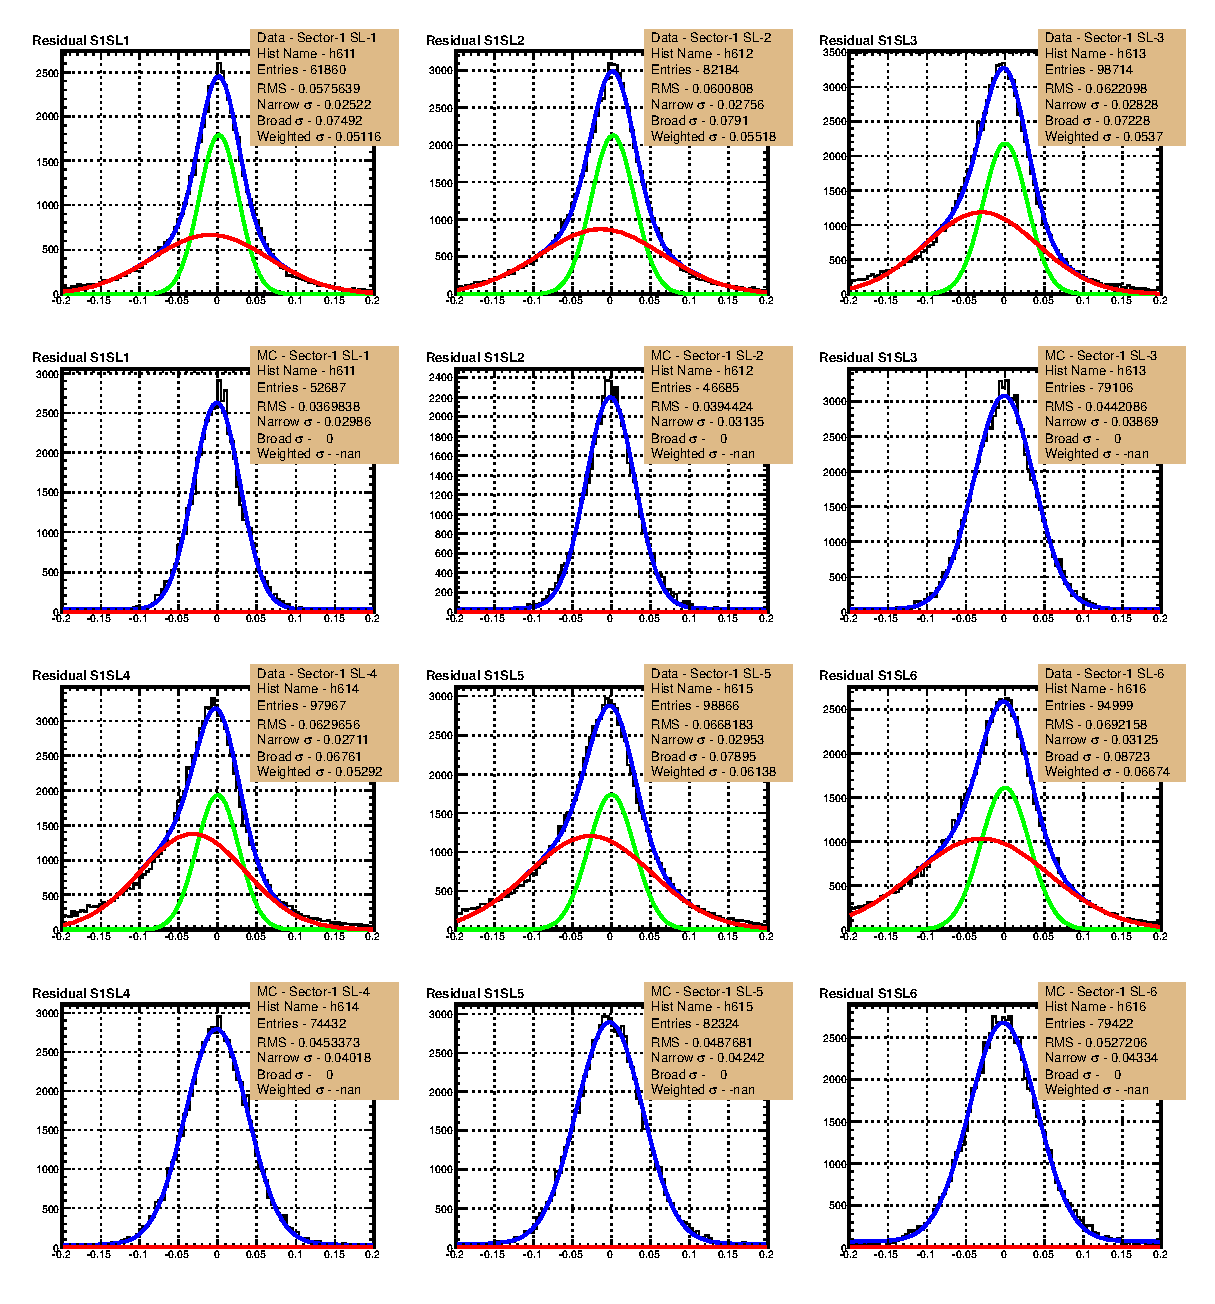
\includegraphics[width=\columnwidth]{figures/calib/dc/Sector_1_compare_default.eps}
\caption[DC superlayers Resolution Matching]{\label{fig:SLRes_default}Plots and Fits used to compare the residuals (resolution) for Drift Chamber superlayers in CLAS Sector 1, between the Data and the Simulation using the default GPP smearing.}
\end{center}\end{figure}

\begin{figure}[htpb]\begin{center}
\begin{subfigure}{0.47\columnwidth}
    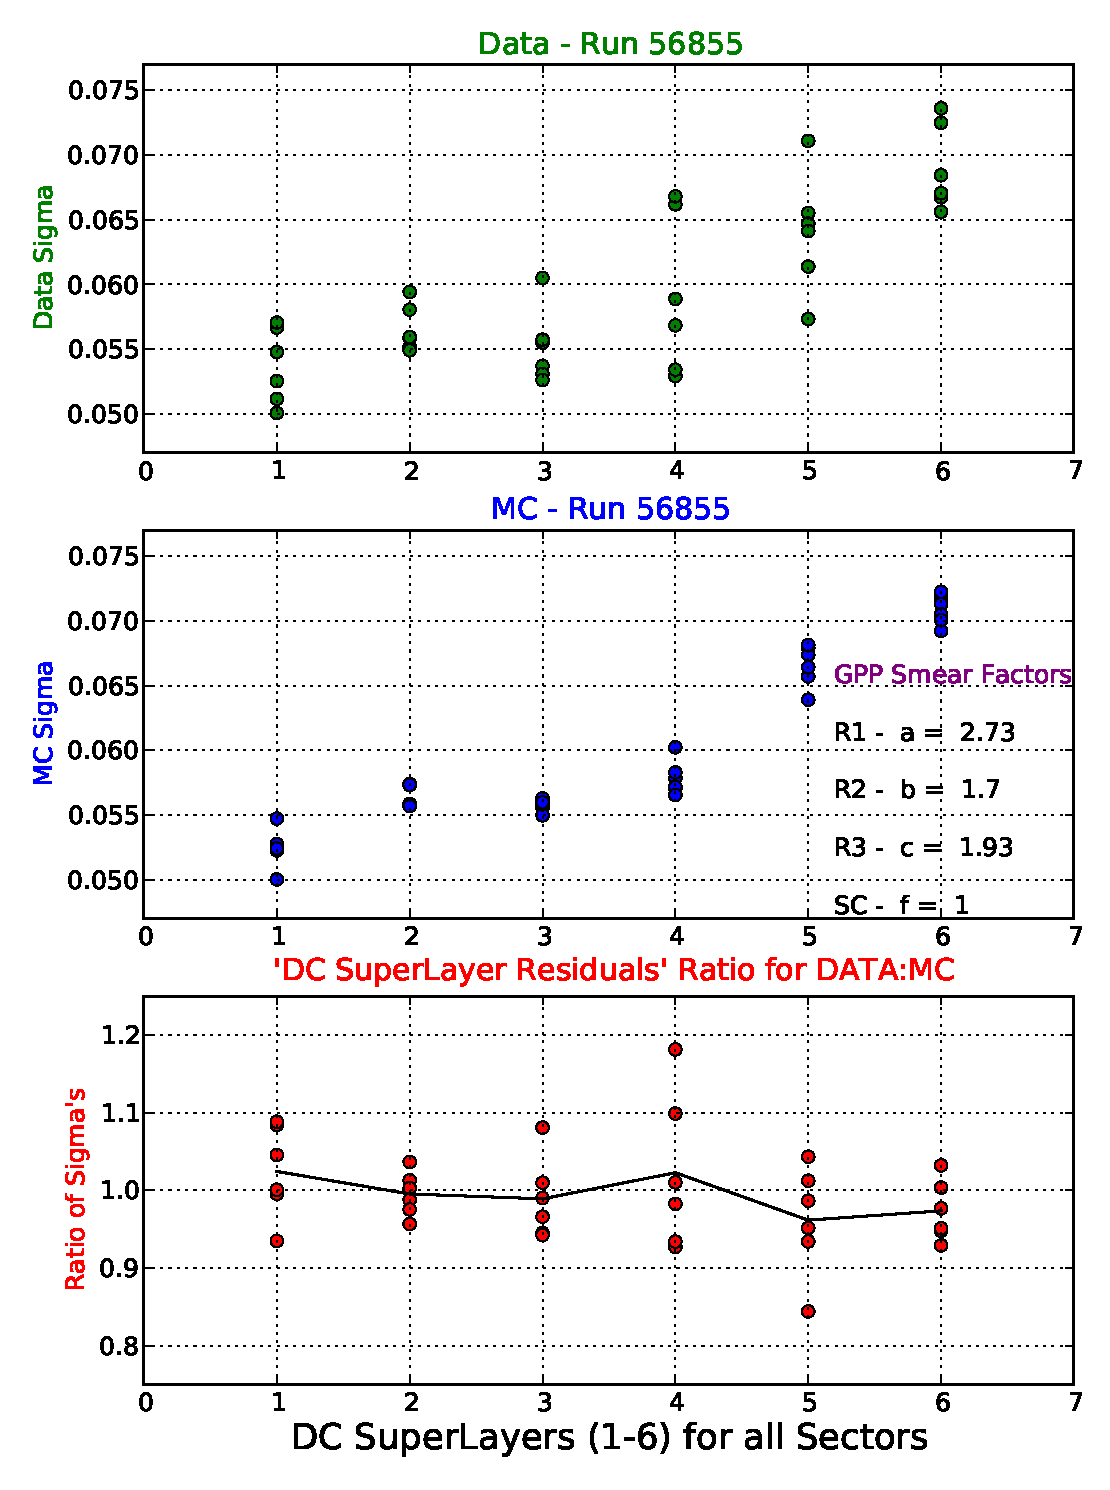
\includegraphics[width=\columnwidth]{figures/calib/dc/DC_Sigma_SL.eps}
    \label{fig:DC_SL_best}
\end{subfigure}
\begin{subfigure}{0.47\columnwidth}
    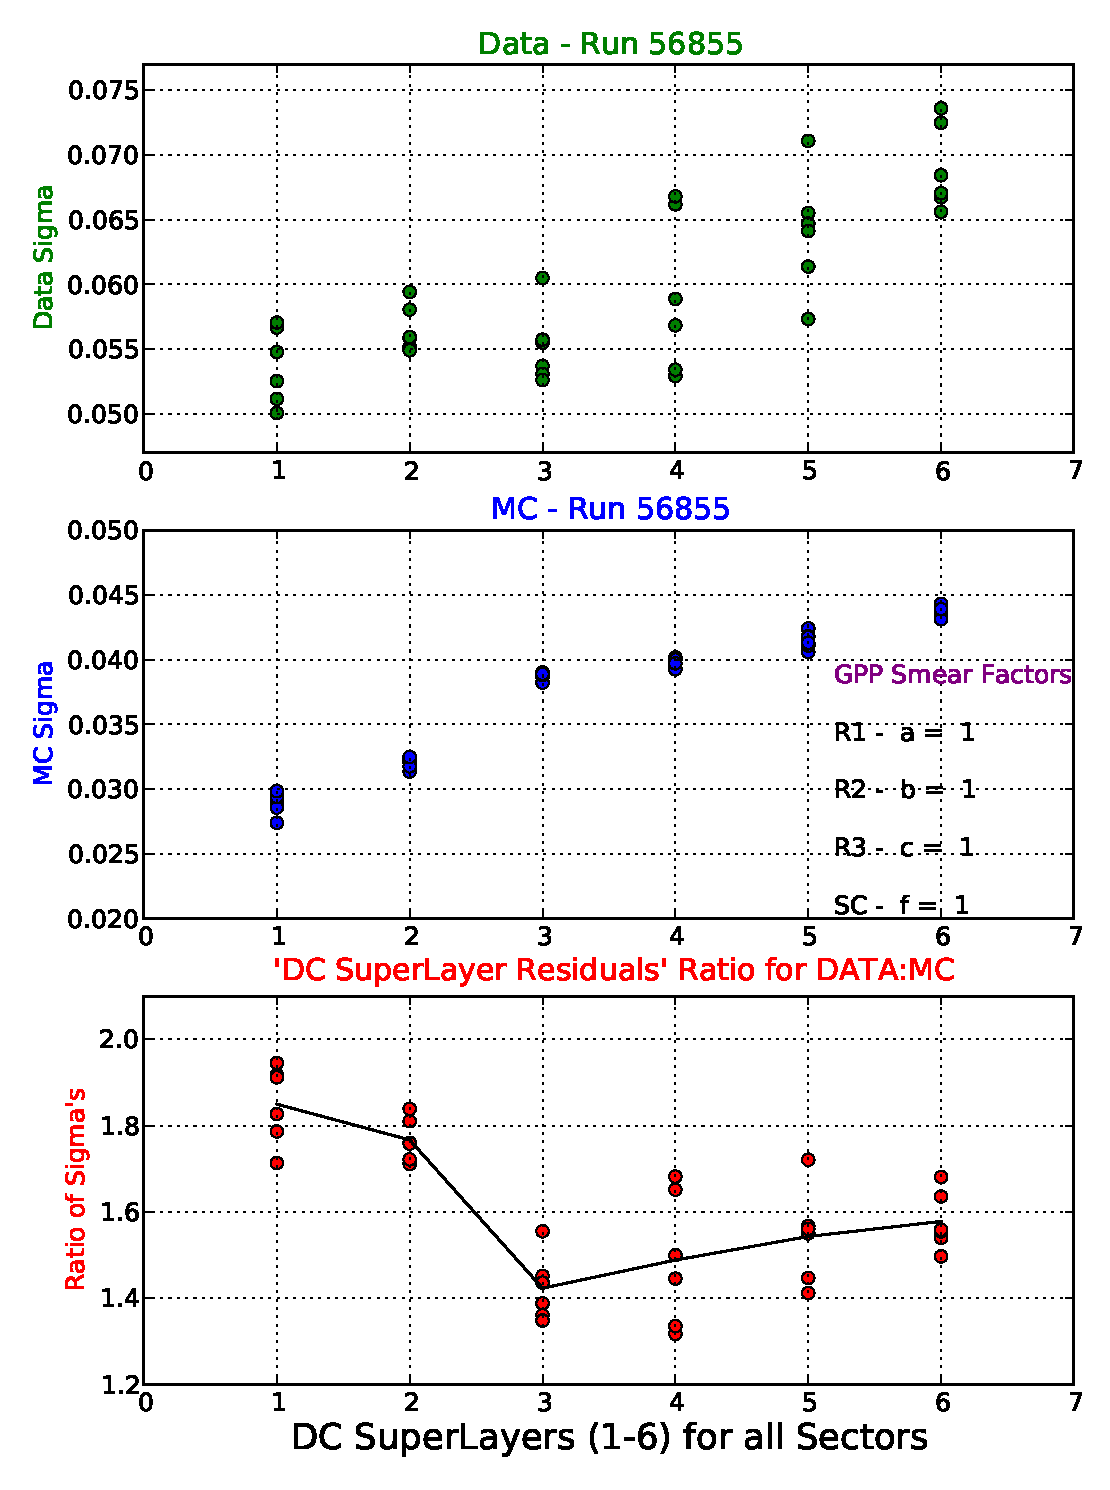
\includegraphics[width=\columnwidth]{figures/calib/dc/DC_Sigma_SL_default.eps}
    \label{fig:DC_SL_default}
\end{subfigure}
\caption[DC superlayers Resolution Matching]{\label{fig:DC_SL_Match}Comparison of the DC residuals on a superlayer basis for all the CLAS sectors for real as well as simulated events. The left plots use the best estimated smearing parameters for the DC DOCA to match the real and simulated data shown in Figure~\ref{fig:SLRes}., whereas the right plots use the default GPP smearing shown in Figure~\ref{fig:SLRes_default}.}
\end{center}\end{figure}

The smearing parameter `-f' for the Time of Flight timing resolution is one of the GPP parameters that is usually used to match the quality of data and simulation. Using the reference run 56855, we observe that the default GPP smearing is adequate (see Figure \ref{fig:TOF_Res}).

\begin{figure}[htpb]\begin{center}
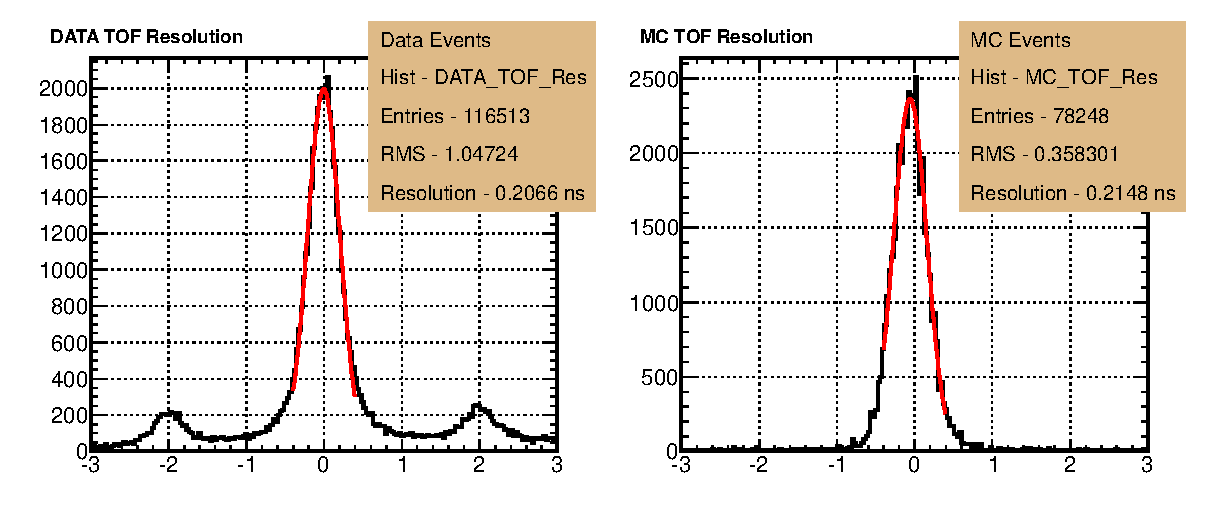
\includegraphics[width=\columnwidth]{figures/calib/dc/TOF_Compare.eps}
\caption[TOF Resolution Matching]{\label{fig:TOF_Res}Plots and Fits used to match the TOF timing resolution. The default smearing of GPP was found to be adequate in this case.}
\end{center}\end{figure}

These smearing parameters affect the reconstruction efficiency for the tracks in CLAS during simulations. A rudimentary analysis quantifying the effect is presented in Table~\ref{tab:recon.eff}. As expected, as the Drift chamber response becomes more noisy due to smearing of DOCA (higher DC residuals), the reconstruction and tracking efficiency in CLAS goes down.

\begin{table}
\begin{center}
\begin{minipage}{\textwidth}
\caption{\label{tab:recon.eff} Measure of Track Reconstruction Efficiency for sets of \texttt{gpp} parameters}
\begin{center}
\begin{tabular}{ccccccc}
\hline \hline
Events & Events & Reconstruction & \multicolumn{4}{c}{\prog{gpp} Smearing Factors} \\
Generated  &  Accepted  & Acceptance & -a & -b & -c & -f \\
\hline
90000 & 1217 & 1.352\% & 1     & 1   & 1    & 1 \\
90000 & 1161 & 1.29\%  & 2.73  & 1.7 & 1.93 & 1 \\
90000 & 1053 & 1.17\%  & 2.73  & 1.7 & 1.93 & 2 \\
\hline \hline
\end{tabular}
\end{center}
\end{minipage}
\end{center}
\end{table}

\subsection{\label{sec:sim.recon}Reconstruction of Simulated Data}

The reconstruction of simulated data requires a slightly different tracking function and is taken care of by adding the option \verb+-X0+ to the reconstruction program. For protons, pions and kaons:
\begin{verbatim}
a1c -T4 -ct1930 -cm0 -cp0 -X0 -d1 -F -P0x1bff -z0,0,-90 \
    -Aprlink_tg-90pm30.bos -oevents.a1c events.gpp
\end{verbatim}
and for electrons and positrons:
\begin{verbatim}
a1c -R10 -T4 -ct1930 -cm0 -cp0 -X0 -d1 -F -P0x1bff -z0,0,-90 \
    -Aprlink_tg-90pm30.bos -oevents.a1c events.gpp
\end{verbatim}
The help output of \prog{a1c} says this about the \verb+-X#+ option:
\begin{verbatim}
    [-X#]    use a different x vs. t function in tracking (def = 2, MC = 0)
\end{verbatim}

\FloatBarrier

\subsection{\label{sec:fiducial}Fiducial Region Selection}

\subsection{Simulating the Lepton Trigger}\label{sec:analysis.accept.trigger}
During the collection process, for an event to be written by the \abbr{DAQ} it must have passed at least one of the trigger ``bits" defined in Sec.~\ref{sec:summary.trigger}. The process of lepton triggering required a coincidence between the \abbr{EC} and the \abbr{CC} subsystems. This coincidence was established by using the voltage sum of the \abbr{CC} for a sector and the voltage sum of the \abbr{EC} for the same sector and comparing each sum to a preset threshold described in Table~\ref{tab:data.ecccthresh}. However when \abbr{GSIM} simulates tracks through the \abbr{CC} and \abbr{EC}, it does not account for the minimum voltage threshold that was required for data collection, moreover the simulation of the trigger must match the trigger efficiency seen for a selected reaction, i.e. the lepton trigger efficiency for $\pi^0$ candidates discussed in~\cite{clas.thesis.kunkel}.

Simulation of the \abbr{CC} and \abbr{EC} trigger ``bit 6'', Table~\ref{tab:data.trig.conf.2}, was performed by writing an algorithm that attempted to mimic the method in which triggered data was recorded. To accomplish this a modified function, written by Simeon McAleer from FSU, was written into the simulation reconstruction algorithm. The routine returned the sector and a boolean of 0 or 1 (pass or fail), that simulated the trigger based on the following criteria;
\begin{enumerate}\label{trig:sim.all}
\item The sector with the highest EC summed energy over threshold. \label{trig:sim.ECtot} 
\item The sector with the highest EC Inner Layer summed energy over threshold. \label{trig:sim.ECinner} 
\item The sector with the highest CC summed energy over threshold. \label{trig:sim.CCtot} 
\item All three above conditions must be in same sector.
\end{enumerate}
Thresholds as described in Table~\ref{tab:data.ecccthresh} are 80~mV, 60~mV and 20~mV for \abbr{EC} \emph{inner}, \abbr{EC}\emph{total} and CC respectively. The \abbr{CC} trigger threshold was applied to groups of eight \abbr{CC} \abbr{PMT}s, called ``sim bits''. The ``sim bits'' were staggered by four \abbr{PMT}s so that each \abbr{PMT} goes into two ``sim bits'', after which all ``sim bits'' were ``\emph{OR}'''d together. If any ``sim bit'' calculated as above threshold, that specific sector was then compared to the remaining sectors to establish the condition listed in~\ref{trig:sim.CCtot}.

The \abbr{EC} \emph{inner} and \abbr{EC} \emph{total} trigger thresholds were applied to all \abbr{EC} strips in a sector. This was done by summing over the energy for every strip in every orientation of the \abbr{EC} per sector. If the energy summation for the \abbr{EC} \emph{inner} was above threshold,   that specific sector was then compared to the remaining sectors to establish the condition listed in~\ref{trig:sim.ECinner}. If the energy summation for the \abbr{EC} \emph{total} was above threshold, that specific sector was then compared to the remaining sectors to establish the condition of the sector with the highest EC summed energy over threshold.

\subsubsection{Validity of Trigger Simulation}
The actual triggered data could have been triggered by the following sceneries;
\begin{enumerate}\label{trig:get.all}
\item $e^-$ \abbr{CC} and \abbr{EC} hit above preset thresholds,
\item $e^+$ \abbr{CC} and \abbr{EC} hit above preset thresholds,
\item $e^-$ \abbr{CC} hit above preset thresholds and $e^+$ \abbr{EC} hit above preset thresholds in the same sector, 
\item $e^-$ \abbr{EC} hit above preset thresholds and $e^+$ \abbr{CC} hit above preset thresholds in the same sector. 
\end{enumerate}
The lepton trigger ``bit 6" was 100\% efficient, for $\pi^0$ candidates (see~\cite{clas.thesis.kunkel} Sec. \textit{\textbf{Lepton Trigger Efficiency for $\pi^0$ Candidates}}), when the data was cut using all the conditions listed above (1, 2, 3, 4) using an ``OR" flag. This means that a $\gamma p \to p e^+ e^-$ event must satisfy at least one of the listed conditions. The reduction in events when at least one of the conditions was satisfied was 69.91\%. Prior to simulating the trigger, cutting the \abbr{MC} with the listed conditions reduced the event yield by 81.91\%. Simulating the trigger and cutting on the \abbr{MC} events with the listed conditions reduced that event yield to 69.48\%. This indicates that the trigger simulation is properly mimicking the trigger configuration used when data is collected. 

%actual physics events recorded by \abbr{CLAS}.
%
%
%When all the conditions listed above are compared together using an ``\emph{OR}'' flag, on \piz data, 69.91\% of events remain. To check the validity of the trigger simulation, events from the \piz reconstructed simulation were placed under the conditions as the actual data. Without placing the boolean of 1 on the simulation, 81.91\% of events remain. Placing the boolean of 1 on the simulation, 69.48\% of events remain, indicating the trigger simulation is mimicking the actual physics events recorded by \abbr{CLAS}. 





